\chapter{Simulation}
This chapter discusses some simulation results, using a simple mathematical model to create a controller. First the mathematical model is discussed, after that the simulation results are discussed and compared with the internal Matlab solvers.

\section{Model complexity}
The trailer model has a very low computational complexity, which makes it cheap to simulate with. The quad copter model, is a very complex model, that requires lots of computations for each simulation step. In this chapter it will become clear that PANOC is a very good with simple models, but a significantly slower with complex models compared to a interior point method.


\section{Trailer model}
The trailer model is illustrated in figure~\ref{fig:trailer model}, the left rectangle is the trailer and the right rectangle is the driver. The driver pulls the trailer forward. The driver is connect to the trailer via a single arm as illustrated in figure~\ref{fig:trailer model}. The control system can only change the speed in the Y and X axis. The goal of the control system is to get the trailer at a certain position and at a certain angle. Figure shows the trailer in a neutral position, so under an angle of 0 degrees.

\begin{figure}
	\centering
	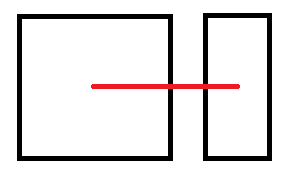
\includegraphics[width=0.5\textwidth]{trailer}
	\caption{trailer}
	\label{fig:trailer model}
\end{figure}

The mathematical model of the trailer is represented in equation~\ref{eq:trailer model}, $u_x$ and $u_y$ are the inputs of the system and represent the speed in the Y and X direction. The angle is represented by $\theta$ , the distance between the driver and the trailer is represented by L. The position of the trailer is represented by $p_x$ and $p_y$.

\begin{equation}
	\begin{cases}
		\dot{p_x} = u_x + L sin \theta \cdot \dot{\theta} \\
		\dot{p_y} = u_y + L cos \theta \cdot \dot{\theta} \\
		\dot{\theta} = \frac{1}{L}(u_ycos \theta - u_x sin \theta)	
	\end{cases}
	\label{eq:trailer model}
\end{equation}

\section{A simple trailer example}
A simple way of measuring the performance of the library is to compared it to the alternatives. In the following simulation the nmpc-codegen library will be compared to, ForBes zerofrp2 the Matlab implementation of the panoc algorithm. And to the internal Matlab function fmincon using either of the tree algorithms interior point,SQP and active set.

\subsection{General performance}
Several NMPC problems can be constructed and solved with nmpc-codegen. Figure~\ref{fig:demos} illustrates the problems used to benchmark nmpc-codegen, they all use the simple trailer model but have different obstacles. The time till convergence is measured, the average time is displayed in table~\ref{tbl:mean time till convergence} in the appendix. While the maximum and minimum time is displayed in the appendix: table~\ref{tbl:min time till convergence} and table~\ref{tbl:max time till convergence}.

The convergence time can be expresses relatively to the convergence time of the nmpc-codegen time as illustrated by equation~\ref{eq:definition relative time}. These results are displayed in table~\ref{tbl:mean relative time till convergence}. From table~\ref{tbl:mean relative time till convergence} it's clear that nmpc-codegen dominates by a significant margin.

\begin{equation}
	t_{relative} = \frac{t_{algorithm}}{t_{nmpc-codegen}}
	\label{eq:definition relative time}
\end{equation}

\subsection{In-dept analysis of performance}
The in-dept simulation contains four circular obstacles, the trailer will move from the lower left corner to the upper right corner. Each of the algorithms will calculate the optimal path up to the tolerance of $10^{-3}$. The input for one step is then applied to the system equation, and the next state is obtained. The same nmpc problem is solved using the new state as current state  and the new input is applied again.

The state of the trailer will is represented by arrows, the starting point of the arrow is the position of the trailer. The angle of the arrow represents the positional angle of the trailer. The amplitude of the arrow has no meaning.

Figure~\ref{fig:solution path trailer example} contains the results of the simulation. The panoc algorithm calculated the lowest located path while all three of the fmincon algorithms opted for the upper located path. Both of these paths are valid solutions. It is immediately clear from figure~\ref{fig:timings trailer example} that the nmpc-codegen library is significantly faster. The other four algorithm's are about the same for the first 30 steps, after about 30 steps the ForBes zerofpr2 algorithm is faster then either of the tree fmincon algorithms.

The nmpc-codegen library uses a cautious lbfgs update which improves the performance of the lbfgs. This is clear from figure~\ref{fig:iterations trailer example} where not the time to convergence but iterations till convergence are illustrated. The nmpc-codegen clearly needs less iterations than theForbes zerofpr2. As the simulation progresses, less and less iterations are needed to calculate optimal solution. And the lbfgs doesn't influence the convergence as much, so the two algorithms have about the same amount iterations till convergence.
\begin{figure}[H]
	\centering
	\begin{subfigure}[b]{0.45\textwidth}
		\centering
		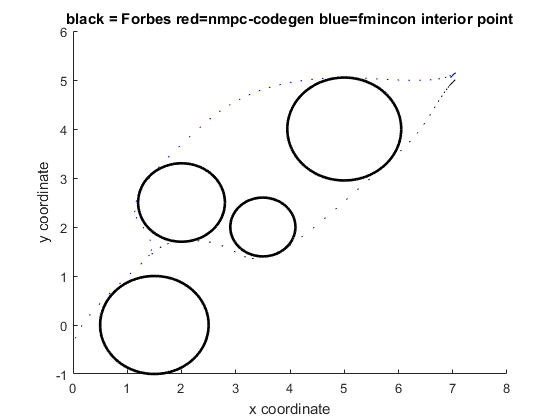
\includegraphics[width=1.2\textwidth]{compare_libs/path}
		\caption{path}
		\label{fig:solution path trailer example}
	\end{subfigure}
	
	\begin{subfigure}[b]{0.45\textwidth}
		\centering
		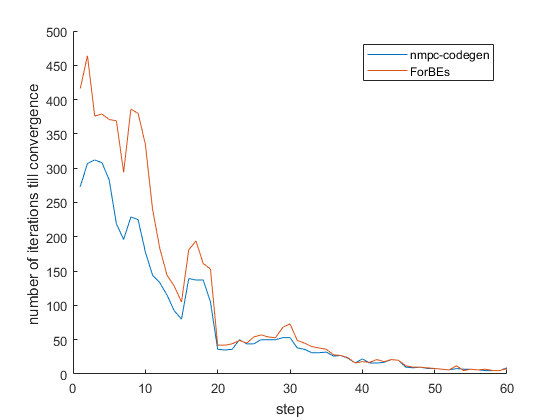
\includegraphics[width=1.2\textwidth]{compare_libs/iterations}
		\caption{iterations}
		\label{fig:iterations trailer example}
	\end{subfigure}
	\hfill
	\begin{subfigure}[b]{0.45\textwidth}
		\centering
		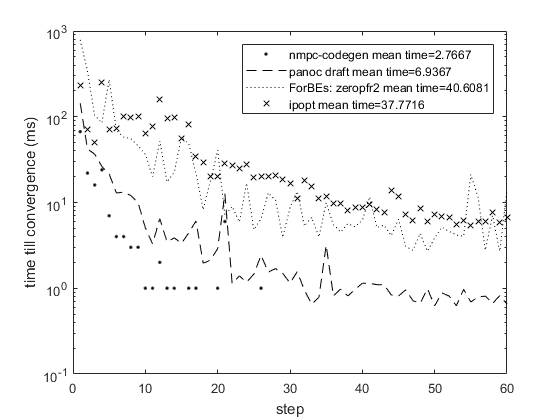
\includegraphics[width=1.2\textwidth]{compare_libs/timings}
		\caption{timings}
		\label{fig:timings trailer example}
	\end{subfigure}
	\caption{Schematic representation of the software}
\end{figure}

\section{Quadcopter model}
%TODO: reference source model !!!!!!!!!!!!!!!!!!
The invention of electronic control systems has proven to be especially useful when controlling quadcopters. Because of their complex behavior they are hard to control manually by a pilot. However quadcopters are popular among unmanned aerial vehicles but they are controlled by a fast digital/analog controller.

\subsection{Mathematical model}
The behavior of a quad copter is described by a set of nonlinear equations as illustrated in equation~\ref{eq:mathematical model quadcopter}.

\begin{table}[]
	\centering
	\caption{constants used in quadcopter model}
	\label{btl:quadcopter model constants}
	\begin{tabular}{|l|l|l|l|}
		\hline
		Parameter                               & Symbol   & Value             & Unit           \\ \hline
		Mass of the quadcopter                  & m        & 0.5               & kg             \\
		Radius of the quadcopter                & L        & 0.25              & m              \\
		Propeller lift coefficient              & k        & $3 \cdot 10^{-6}$ & $Ns^2$        \\
		Propeller drag coefficient              & b        & $1 \cdot 10^{-7}$ & N m $s^2$      \\
		Acceleration of gravity                 & g        & 9.81              & m/$s^2$        \\
		Air friction coefficient                & $k_d$    & 0.25              & kg/s           \\
		Quadcopter inertia about the $x^b$-axis & $I_{xx}$ & $5 \cdot 10^{-3}$ & kg $m^2$       \\
		Quadcopter inertia about the $y^b$-axis & $I_{yy}$ & $5 \cdot 10^{-3}$ & kg $m^2$       \\
		Quadcopter inertia about the $z^b$-axis & $I_{zz}$ & $1 \cdot 10^{-2}$ & kg $m^2$       \\ 
		Motor constant                          & $c_m$    & $1 \cdot 10^{4}$  & $v^{-2}s^{-2}$ \\
		\hline
	\end{tabular}
\end{table}

\begin{equation}
	\begin{aligned}
		\dot{x} &= v_x \\
		\dot{y} &= v_y \\
		\dot{z} &= v_z \\
		\dot{v_x} &= -\frac{k_d}{m}v_x + \frac{k \cdot c_m}{m}\Big(sin(\gamma)sin(\phi)+cos(\gamma)cos(\phi)sin(\theta)\Big)\Big(u_1 + u_2 + u_3 + u_4\Big) \\
		\dot{v_y} &= -\frac{k_d}{m}v_y + \frac{k \cdot c_m}{m}\Big(cos(\phi)sin(\gamma)sin(\theta)-cos(\gamma)sin(\phi)\Big)\Big(u_1 + u_2 + u_3 + u_4\Big) \\
		\dot{v_z} &= -\frac{k_d}{m}v_y -g + \frac{k \cdot c_m}{m}\Big(cos(\theta)cos(\phi)\Big)\Big(u_1 + u_2 + u_3 + u_4\Big) \\
		\dot{\phi} &= \omega_x + \omega_y\Big( sin(\phi)tan(\theta) \Big) + \omega_z \Big( cos(\phi) tan(\theta) \Big) \\
		\dot{\theta} &= \omega_y cos(\phi) - \omega_z sin(\phi) \\
		\dot{\gamma} &= \frac{sin(\phi)}{cos(\theta)}\omega_y + \frac{cos(\phi)}{cost(\theta)} \omega_z \\
		\dot{\omega_x} &= \frac{Lkc_m}{I_{xx}}\Big( u_1 - u_3 \Big) - \Big( \frac{I_{yy}-I_{zz}}{I_{xx}} \Big) \omega_y \omega_z\\
		\dot{\omega_y} &= \frac{Lkc_m}{I_{yy}}\Big( u_2 - u_4 \Big) - \Big( \frac{I_{zz}-I_{xx}}{I_{yy}} \Big) \omega_x \omega_z\\
		\dot{\omega_z} &= \frac{bc_m}{I_{zz}}\Big( u_1 - u_2 + u_3 - u_4 \Big) - \Big( \frac{I_{xx}-I_{yy}}{I_{zz}} \Big) \omega_x \omega_y\\
	\end{aligned}
	\label{eq:mathematical model quadcopter}
\end{equation}

\subsection{Simulation results}
Figure~\ref{fig:Simulation results with quadcopter} contains a simple simulation with the quad copter model, the path is displayed in figure~\ref{fig:solution path trailer quad}. The two sphere shaped obstacles, and the quad copter is moving from the star symbol to the circle. The time to convergence of each step of the simulation, is displayed in figure~\ref{fig:timings trailer quad}.

As mentioned at the start of this chapter, the quad copter model computational expensive model. This means that the computational cost of solving a system, is more in line with the computational cost of simulating one step of the system. 

A interior point method, must solve a system at each step of the algorithm. The interior method used from ipopt solves the system directly with a computational cost of about $\mathcal{O}(n^3)$ . While PANOC only has to cope additional cost of about $\mathcal{O}(Ln)$ with L as the buffer size.  because the L-BFGS algorithm only uses inner products and vector additions.

This means that the difference between PANOC and ipopt is rather small with the quad copter model. Which is clearly visible, in figure~\ref{fig:timings trailer quad}, where the ipopt line is very near the ipopt line.
\begin{figure}[H]
	\centering
	\begin{subfigure}[b]{0.45\textwidth}
		\centering
		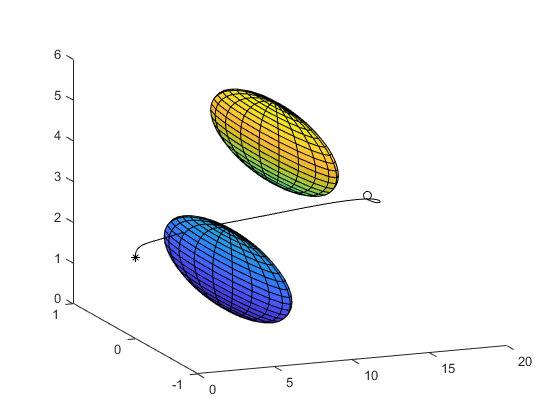
\includegraphics[width=1.2\textwidth]{compare_libs/path_quad}
		\caption{path}
		\label{fig:solution path trailer quad}
	\end{subfigure}
	\hfill
	\begin{subfigure}[b]{0.45\textwidth}
		\centering
		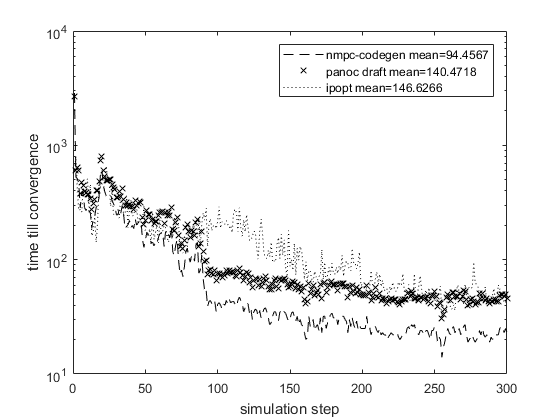
\includegraphics[width=1.2\textwidth]{compare_libs/timings_quad}
		\caption{timings}
		\label{fig:timings trailer quad}
	\end{subfigure}
	\caption{Simulation results with quadcopter}
	\label{fig:Simulation results with quadcopter}
\end{figure}

\section{Influence of noise}
Until now all simulations were executed without any kind of noise. However in reality there is always some kind of state noise. So is essential to study how PANOC handles state noise.

The white noise has a maximum amplitude of 0.1 on the x state and the y state. It has a amplitude of 0.05 on the angle $\theta$. The double noise simply doubles the maximum amplitude of the noise. This way the influence of the size of the noise can be studied.

Figure~\ref{fig:Noise simulations with the trailer model} contains the simulation results using PANOC or ipopt as solver. Going from no state noise to a bit of state noise makes a significant difference when solving with PANOC. The interior point method from ipopt, thus take longer to converge when noise is added. However it is less proportional towards the noise, as the interior point method here uses a direct method to solve the system.

\begin{figure}[H]
	\centering
	\begin{subfigure}[b]{0.45\textwidth}
		\centering
		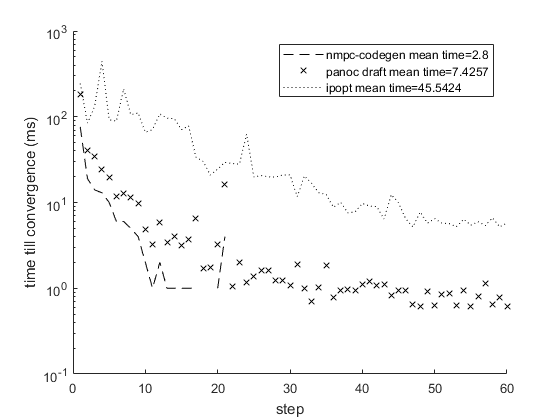
\includegraphics[width=1.2\textwidth]{compare_libs/trailer_without_noise}
		\caption{without noise}
		\label{fig:timings trailer without noise}
	\end{subfigure}
	\hfill
	\begin{subfigure}[b]{0.45\textwidth}
		\centering
		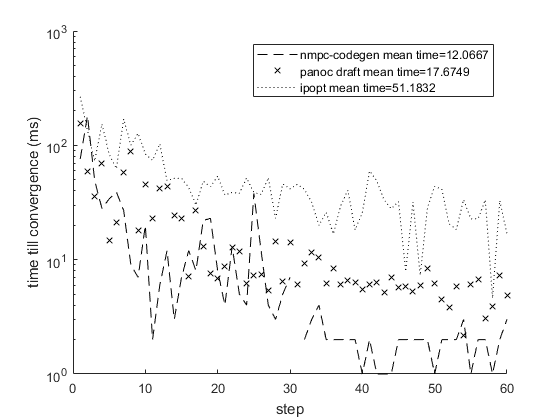
\includegraphics[width=1.2\textwidth]{compare_libs/trailer_with_noise}
		\caption{with noise}
		\label{fig:timings trailer with noise}
	\end{subfigure}
	\begin{subfigure}[b]{0.45\textwidth}
		\centering
		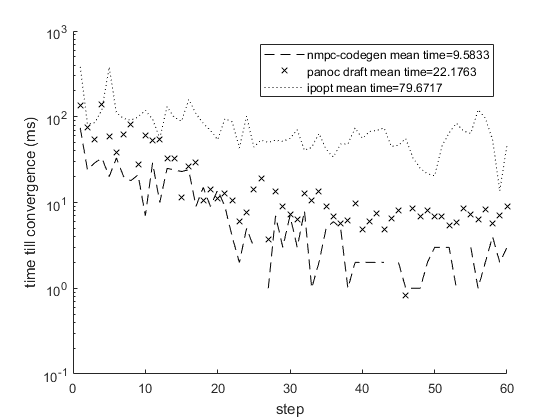
\includegraphics[width=1.2\textwidth]{compare_libs/trailer_with_double_noise}
		\caption{with double noise}
		\label{fig:timings trailer with double noise}
	\end{subfigure}
	\hfill
	\begin{subfigure}[b]{0.45\textwidth}
		\centering
		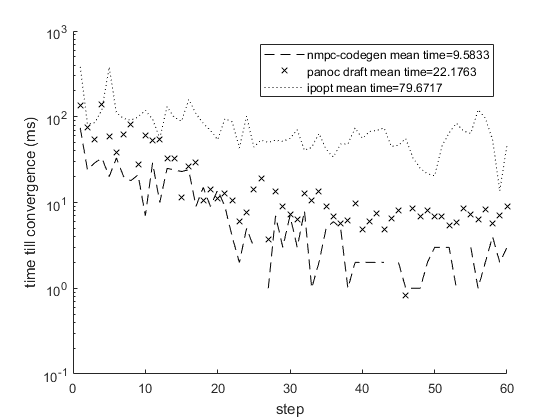
\includegraphics[width=1.2\textwidth]{compare_libs/trailer_with_double_noise}
		\caption{path without noise}
		\label{fig:path noise simulations}
	\end{subfigure}
	\caption{Noise simulations with the trailer model}
	\label{fig:Noise simulations with the trailer model}
\end{figure}

\begin{table}[H]
	\centering
	\begin{tabular}{|l|c|c|c|c|}
		\hline
		&\textbf{no noise}&\textbf{with noise}&\textbf{double noise}\\\hline
		\textbf{nmpc-codegen}&3 ms&12 ms&10 ms \\\hline
		\textbf{draft panoc}&8 ms&18 ms&22 ms \\\hline
		\textbf{OPTI:ipopt}&45 ms&51 ms&80 ms \\\hline
	\end{tabular}
	\caption{average till convergence in miliseconds}
	\label{tbl:average till convergence noise}
\end{table}

% only do simulations with trailer model, quadcopter models goes nuts
% 2 figures , one with noise and one without use draft PANOC with ipopt
%TODO add simulation with noise

\section{Problem with local minimum}
One problem with the approach discussed in this chapter, it's visible in the third demo. The results of the third demo are illustrated in figure~\ref{fig:demo: local minimum problem}, the trailer drives through the obstacle which is obviously impossible in reality. In reality the trailer will simply crash into the obstacle, and get stuck. Of course it is possible to increase the weight on the obstacle, this will make the problem harder. As the condition will get worse, and the solution will be about the same. The trainer will get stuck against the obstacle.

\begin{figure}[H]
	\centering
	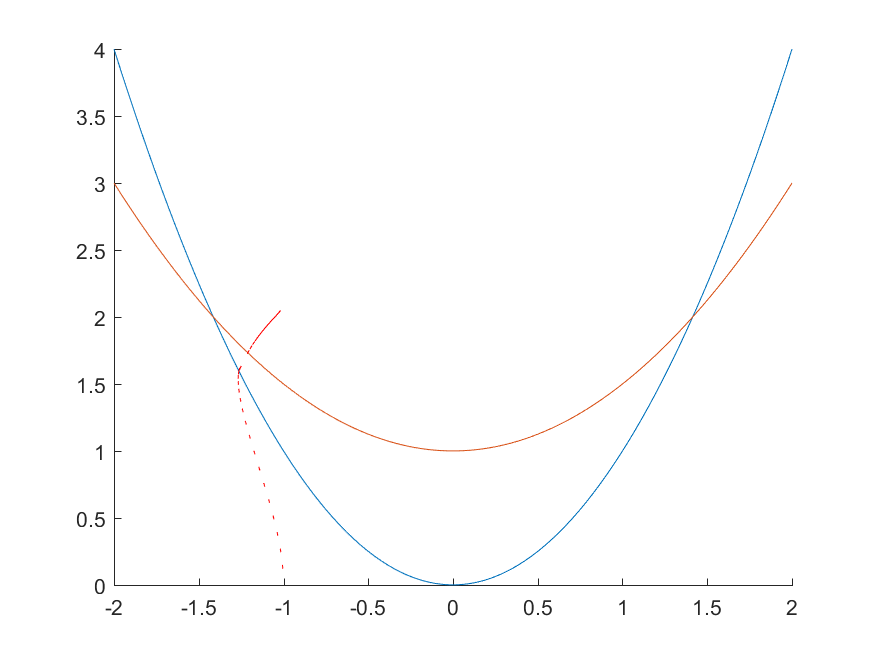
\includegraphics[width=0.5\textwidth]{demos/demo3}
	\caption{Local minimum problem}
	\label{fig:demo: local minimum problem}
\end{figure}

\section{Conclusion}

The simulations clearly indicate that a great speed up his gained by implementing the panoc algorithm in C. As the algorithm doesn't require a lot of memory it can be run efficiently on small embedded devices. The control engineer can design and test the performance of the algorithm in either Matlab or Python.

